\documentclass[UTF8]{article}

% \usepackage{indentfirst} %缩进
% \usepackage{xeCJK}    %使用系统字体
\usepackage{ctex}
\usepackage{fancyhdr} %自定义页眉页脚
\usepackage{listings} %source code
\usepackage{tabu}
\usepackage{booktabs}
\usepackage{graphicx}
\usepackage{multirow}

% \setCJKmainfont{SimSun} %设置 CJK 主字体为 SimSun (宋体)
% \pagestyle{empty}                   %不设置页眉页脚
% \usepackage{amsmath, amsthm, amssymb, amsfonts} %数学公式
% \usepackage[a4paper,left=3cm,right=3cm,top=3cm,bottom=3cm]{geometry}
% %\usepackage[tmargin=1in,bmargin=1in,lmargin=1.25in,rmargin=1.25in]{geometry}.
% \usepackage{booktabs} %插入表格
% \usepackage[section]{placeins} %避免浮动
% \usepackage{listings} %插入代码
% \usepackage{ctex}     %中文宏包
% \usepackage[svgnames, table]{xcolor} %彩色表格
% \usepackage{algorithm}          %伪代码
% \usepackage{algorithmicx}
% \usepackage{algpseudocode}
% \usepackage{algorithm,algpseudocode,float}
% \usepackage{lipsum}
% \usepackage{enumitem}           %调整列举环境
% \usepackage{url}
% \usepackage{fontspec,xunicode}

% %-----------------------xeCJK下设置中文字体------------------------------%
% \setCJKfamilyfont{song}{SimSun}                             %宋体 song
% \newcommand{\song}{\CJKfamily{song}}
% \setCJKfamilyfont{fs}{FangSong}                      %仿宋  fs
% \newcommand{\fs}{\CJKfamily{fs}}
% \setCJKfamilyfont{ktgb}{KaiTi}                      %楷体2312 ktgb
% \newcommand{\ktgb}{\CJKfamily{ktgb}}
% \setCJKfamilyfont{yh}{Microsoft YaHei}                    %微软雅黑 yh
% \newcommand{\yh}{\CJKfamily{yh}}
% \setCJKfamilyfont{hei}{SimHei}                              %黑体  hei
% \newcommand{\hei}{\CJKfamily{hei}}
% \setCJKfamilyfont{hwxk}{STXingkai}                                %华文行楷  hwxk
% \newcommand{\hwxk}{\CJKfamily{hwxk}}

% \newcommand{\shiyanbaogao}{\fontsize{36pt}{\baselineskip}\selectfont}
% \newcommand{\chuhao}{\fontsize{42pt}{\baselineskip}\selectfont}     %初号
% \newcommand{\xiaochuhao}{\fontsize{36pt}{\baselineskip}\selectfont} %小初号
% \newcommand{\yihao}{\fontsize{28pt}{\baselineskip}\selectfont}      %一号
% \newcommand{\erhao}{\fontsize{21pt}{\baselineskip}\selectfont}      %二号
% \newcommand{\xiaoerhao}{\fontsize{18pt}{\baselineskip}\selectfont}  %小二号
% \newcommand{\sanhao}{\fontsize{15.75pt}{\baselineskip}\selectfont}  %三号
% \newcommand{\sihao}{\fontsize{14pt}{\baselineskip}\selectfont}       %四号
% \newcommand{\xiaosihao}{\fontsize{12pt}{\baselineskip}\selectfont}  %小四号
% \newcommand{\wuhao}{\fontsize{10.5pt}{\baselineskip}\selectfont}    %五号
% % \newcommand{\xiaowuhao}{\fontsize{9pt}{\baselineskip}\selectfont}   %小五号
% % \newcommand{\liuhao}{\fontsize{7.875pt}{\baselineskip}\selectfont}  %六号
% % \newcommand{\qihao}{\fontsize{5.25pt}{\baselineskip}\selectfont}    %七号
\begin{document}


\begin{titlepage}
\center{北京理工大学\underline{计算机}学院2017级}
\vspace{1cm}
\center{\Huge{《数字逻辑》实验二}}
\vspace{0.5cm}
\center{\Huge{实~验~报~告}}
\vspace{2cm}

\begin{center}
\begin{large}
\begin{tabular}{r c}
小组编号& xxxxx\\
\cline{2-2}\\
\hline
学\qquad 号& \hspace{1.7cm}{xxxx} \\
\cline{2-2}\\
姓\qquad 名& 你的名字 \\
\cline{2-2}\\
\hline
学\qquad 号& \hspace{1.7cm}{xxxx} \\
\cline{2-2}\\
姓\qquad 名& 你的名字 \\
\cline{2-2}\\ 
\hline
学\qquad 号& \hspace{1.7cm}{xxxx} \\
\cline{2-2}\\
姓\qquad 名& 你的名字 \\
\cline{2-2}\\ 



% \xiaoerhao{\hei{理论教师}}& \xiaoerhao{\hei{X~X~X}}\\
% \cline{2-2}\\
\end{tabular}
\end{large}
\end{center}
\vfill \hfill
\end{titlepage}
\clearpage


\section{设计题目}

\begin{center}
    
\center{一个三开关的低电压的照明系统}
\end{center}

\paragraph{}
一个低电压的照明系统采用二进制逻辑控制器控制一盏特殊灯的照明,
这盏灯用于T型走廊的交叉口。
在T型走廊的三个端点各有一个控制灯的开关,
这些开关的开合状态决定它们的二进制输出是0还是1,
三个开关分别用$X1$、$X2$和$X3$表示。
这盏灯由一个带缓冲驱动的可控硅控制,
可控硅控制电灯电源电路的导通。当缓冲器的输入$Z$为1的时候,
灯是开着的,当$Z$为0的时候,灯是熄灭的。
你需要得到这样一个函数$Z = F(X1, X2, X3)$,如果任意一个开关变化了,
$Z$的值就会改变,从而控制电灯的开和关。

\section{设计目的}

利用组合逻辑电路,按照题目要求,设计电路模块,
利用三个开关$X1,X2,X3$的输出控制缓冲器输入$Z$,
从而控制一个灯的亮与灭,并结合开发板进行演示验证。

\section{设备器材}
Xilinx Vivado开发环境

EES-338口袋计算机硬件平台,配备 FPGA (XC7A35TCSG324-1C)

\section{设计原理与内容}
\subsection{问题分析}

我们可以由分析得出,输出$Z$同时收$X1,X2,X3$影响,
且当任意一个值发生变化时,Z取反。
我们很快能够联想到格雷码的内容——格雷码就是相邻状态只有一位的改变。

该系统的初始状态为:$X1, X2, X3$都处于关闭状态,故它们的输出都是0。
初始时灯是不亮的,故缓冲器的输入$Z$也是0。
之后,只要任意一个开关的状态改变一次,$Z$的值就会取反。

这就意味着,只要$X1, X2, X3$中输出为1的个数是奇数,
开关状态的改变次数就是奇数,$Z$的值就是1。
这是因为,对于一个开关Xi, 若它的输出是0,则它的状态变化次数为 $2ki$;
若它的输出是1,则它的状态变化次数为$1 + 2ki$。
那么,开关的变化次数,即Z的取反次数为 $2 (k1 + k2 + k3 ) + t$,
其中$ki$为整数,$t$为输出为1的开关个数。
这样一来,该问题就成为了一个偶校验问题。


按照如上分析,可以直接列出真值表,输入按照格雷码排列,则输出从0开始不断取反。
真值表如下:
% TODO 表格

\begin{table}[!htbp]
\centering
\begin{tabu} to 0.8\textwidth{ X[c] | X[c] | X[c] | X[c] }
    \hline
    X1 & X2 & X3 & Z \\
    \hline\hline
    0 & 0 & 0 & 0\\
    0 & 0 & 1 & 1\\
    0 & 1 & 1 & 0\\
    0 & 1 & 0 & 1\\
    1 & 1 & 0 & 0\\
    1 & 1 & 1 & 1\\
    1 & 0 & 1 & 0\\
    1 & 0 & 0 & 1\\

    \end{tabu}
\caption{真值表}
\end{table}
该函数方程即为  

$$Z = X1\oplus X2\oplus X3$$

接下来就可以开始进行组合逻辑电路的设计。

\section{设计步骤}
\subsection{描述需求}

通过开关$X1$, $X2$, $X3$的状态变化,使$Z = X1⊕X2⊕X3$的值变化,
从而使灯亮或灭。

\subsection{定义输入与输出}

定义输入为长度为三位的向量 

\lstset{language=verilog}
\begin{lstlisting}[frame=tb]{somecode}
    [2:0] data_in
\end{lstlisting}

{test}
则\lstinline{data_in[0]},
\lstinline$data_in[1]$ , \lstinline$data_in[2]$分别为开关$X1$, $X2$, $X3$的输出值。
定义输出为\lstinline$data_out$,
其值即为Z的值。

\subsection{程序实现}

在模块streetlight中,使用数据流描述方式,采用\lstinline{assign}对输出进行赋值。可以直接使

用位运算符$\wedge$进行运算,即
\lstset{language=verilog}
\begin{lstlisting}[frame=tb]{somecode}
    data_out = data_in[0]^data_in[1]^data_in[2]
\end{lstlisting}

在测试模块\lstinline{streetlight_tb}中,
定义reg型的变量\lstinline{[2:0] data_in}作为输入端口,
定义wire型的变量\lstinline{data_out}作为输出端口。
然后,将模块streetlight实例化为pj2,
并指定相应的输入和输出。
在initial块中,将0-7的三位二进制数按照格雷码的顺序依次赋值给\lstinline{data_in},
每次赋值之间延迟100个时间单位。

进行RTL分析后,生成RTL原理图:
​
\begin{figure}[htbp]
    \centering
    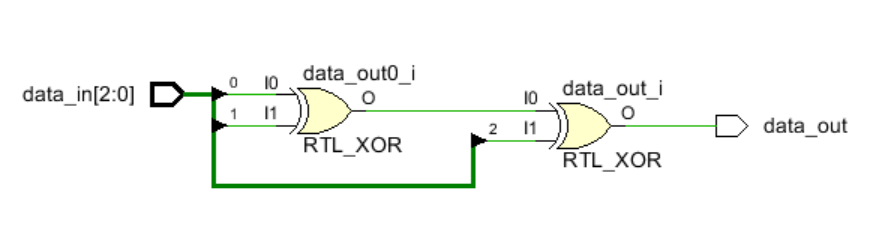
\includegraphics[scale=0.7]{0.png}
    \caption{RTL原理图}
\end{figure}

\subsection{仿真与测试}
进行行为仿真。得到的波形与预计一致。
\subsection{运行}

\section{遇到的问题及解决方法}
\section{参考文献}

\end{document}
